\documentclass[11pt, reqno, letterpaper, twoside]{amsart}
\linespread{1.2}
\usepackage[margin=1.25in]{geometry}

\usepackage{amssymb, bm, mathtools, physics}
\usepackage[dvipsnames,svgnames,table]{xcolor} % 移除 usenames
\usepackage{graphicx} % 移除 [pdftex, xetex]
\usepackage{enumerate, setspace}
\usepackage{float, colortbl, tabularx, longtable, multirow, subcaption, environ, wrapfig, textcomp, booktabs}
\usepackage{pgf, tikz, framed}
\usepackage[normalem]{ulem}
\usetikzlibrary{arrows,positioning,automata,shadows,fit,shapes}
\usepackage[english]{babel}
\usepackage{listings}
\usepackage[final]{microtype}

\lstset{
    language=Python,                % 语言
    basicstyle=\ttfamily\small,     % 字体
    keywordstyle=\color{blue},      % 关键字颜色
    commentstyle=\color{green!50!black}, % 注释颜色
    stringstyle=\color{red},        % 字符串颜色
    showstringspaces=false,         % 不显示空格
    frame=single,                   % 外框
    breaklines=true                 % 自动换行
}

\theoremstyle{plain}
\newtheorem{theorem}{Theorem}

\theoremstyle{definition}
\newtheorem{solution}[theorem]{Solution}

\usepackage{times}

\title{ESE 546\\[0.1in]
Homework 2}
\author{
Jinhao You [you7@seas.upenn.edu]
}



\begin{document}
\maketitle

\begin{solution}[Time spent: 5 hours]
Your solution goes here.\\

\paragraph{\textbf{Problem a}} When BN is placed before ReLU (i.e., Conv → BN → ReLU), which is the standard and widely adopted configuration, BN first normalizes the convolutional output to have zero mean and unit variance, followed by the nonlinear transformation. This arrangement ensures that the inputs to the ReLU are well-conditioned, roughly centered around zero, allowing both positive and negative activations to be preserved. As a result, the network maintains a balanced activation distribution, avoids dead neurons, and exhibits more stable gradients, facilitating faster and more reliable convergence during training.

Conversely, placing ReLU before BN (Conv → ReLU → BN) often degrades performance. Since ReLU truncates all negative activations to zero, the subsequent BN layer receives inputs with a non-symmetric, non-zero-centered distribution. BN then attempts to re-normalize this skewed input, often shifting the zero activations toward negative values, which in turn diminishes the sparsity benefits of ReLU and can lead to reduced representational capacity. Empirically, this configuration tends to slow convergence and decrease overall accuracy. Therefore, the BN-before-ReLU ordering is generally preferred for deep architectures.\\

\paragraph{\textbf{Problem b}} In PyTorch, the functions model.train() and model.eval() are used to switch the model between training and evaluation modes. This distinction is important because some layers behave differently during training and inference. For example, Dropout randomly deactivates a subset of neurons during training to improve generalization, while it is disabled during evaluation so that all neurons contribute to the output. Similarly, Batch Normalization uses the current mini-batch's mean and variance for normalization during training, but relies on the running mean and variance accumulated throughout training when in evaluation mode. 
In HW1, however, our self-implemented library does not include layers such as Dropout or Batch Normalization, meaning that the forward computation remains identical across training and testing. As a result, explicit mode switching using model.train() or model.eval() is unnecessary in this assignment. In contrast, PyTorch is a general-purpose framework that must provide these functions to correctly handle layers whose behavior depends on the model's mode.\\

\paragraph{\textbf{Problem c}} 
The table summarizes the parameter distribution of the network, showing the number of learnable weights in each major block. As depth increases, the number of parameters grows significantly, with most concentrated in the later convolutional layers and the final fully connected layer. 
Batch Normalization layers contain relatively few parameters but help stabilize training. Overall, the network has about 11.69 million parameters in total.\\
\begin{table}[H]
\centering
\small
\setlength{\tabcolsep}{6pt}
\renewcommand{\arraystretch}{1.1}
\resizebox{0.95\textwidth}{!}{
\begin{tabular}{lrrrrrr}
\hline
\textbf{Layer} & \textbf{Conv1} & \textbf{BN1 (w,b)} & \textbf{Conv2} & \textbf{BN2 (w,b)} & \textbf{Downsample} & \textbf{Total} \\
\hline
conv1 & 9,408 & 64, 64 & -- & -- & -- & 9,536 \\
layer1.0 & 36,864 & 64, 64 & 36,864 & 64, 64 & -- & 73,920 \\
layer1.1 & 36,864 & 64, 64 & 36,864 & 64, 64 & -- & 73,920 \\
layer2.0 & 73,728 & 128, 128 & 147,456 & 128, 128 & 8,192 + (128,128) & 229,888 \\
layer2.1 & 147,456 & 128,128 & 147,456 & 128,128 & -- & 295,296 \\
layer3.0 & 294,912 & 256,256 & 589,824 & 256,256 & 32,768 + (256,256) & 1,118,528 \\
layer3.1 & 589,824 & 256,256 & 589,824 & 256,256 & -- & 1,180,416 \\
layer4.0 & 1,179,648 & 512,512 & 2,359,296 & 512,512 & 131,072 + (512,512) & 5,197,584 \\
layer4.1 & 2,359,296 & 512,512 & 2,359,296 & 512,512 & -- & 5,744,128 \\
fc & 512,000 & 1,000 & -- & -- & -- & 513,000 \\
\hline
\textbf{Total parameters} & \multicolumn{6}{r}{11,689,512} \\
\hline
\end{tabular}
}
\caption{Condensed layer-wise parameter summary of the network.}
\label{tab:params-condensed}
\end{table}

\paragraph{\textbf{Problem d}} 
Weight decay serves as a regularization technique that penalizes large parameter values,
making the model smoother, less complex, and less prone to overfitting.
However, the bias parameters behave differently and should not be regularized in the same way.
The bias term mainly helps shift the input distribution of activation functions,
ensuring that neurons operate within appropriate activation regions.
It does not control model complexity and therefore does not contribute to overfitting.

If L2 regularization is applied to the bias term, the bias will be forced toward zero.
This effectively shifts all activation functions back toward the origin
and reduces the model’s ability to adapt to inputs with non-zero means.
As a result, the model may lose flexibility and perform worse on tasks requiring
non-centered input distributions.

Weight decay essentially adds a penalty term to the loss function:
\[
L' = L + \frac{\alpha}{2}\|w\|_2^2
\]
If the bias term is also regularized, the modified loss becomes:
\[
L' = L + \frac{\alpha}{2}(\|w\|_2^2 + b^2)
\]
When the input data are not zero-centered, the model must learn a non-zero bias
to correct the mean offset.
Weight decay, by pushing the bias toward zero, prevents proper adjustment of this shift,
leading to suboptimal training and larger validation error.

\paragraph{\textbf{Problem e}} 
Overall, the BN affine parameters provide per-channel normalization and adaptation, 
while the majority of learnable parameters are concentrated in convolutional and linear weight matrices that determine the model's representational capacity.\\
\begin{table}[H]
\centering
\scriptsize
\setlength{\tabcolsep}{4pt}
\renewcommand{\arraystretch}{1.1}
\resizebox{0.95\textwidth}{!}{
\begin{tabular}{l l}
\hline
\textbf{Category} & \textbf{Representative Parameters (Shape)} \\
\hline
BatchNorm affine parameters &
\begin{tabular}[t]{@{}l@{}}
bn1 (w,b) (64,) \\
layer1.\{0,1\}.bn\{1,2\} (w,b) (64,) \\
layer2.\{0,1\}.bn\{1,2\} (w,b) (128,) \\
layer2.0.downsample.1 (w,b) (128,) \\
layer3.\{0,1\}.bn\{1,2\} (w,b) (256,) \\
layer3.0.downsample.1 (w,b) (256,) \\
layer4.\{0,1\}.bn\{1,2\} (w,b) (512,) \\
layer4.0.downsample.1 (w,b) (512,) \\
\end{tabular} \\[1ex]

Bias parameters (Conv/FC) &
fc.bias (1000,) \\[1ex]

Other parameters (Conv/FC weights) &
\begin{tabular}[t]{@{}l@{}}
conv1.weight (64, 3, 7, 7) \\
layer1.\{0,1\}.conv\{1,2\}.weight (64, 64, 3, 3) \\
layer2.\{0,1\}.conv\{1,2\}.weight (128, *, 3, 3) \\
layer2.0.downsample.0.weight (128, 64, 1, 1) \\
layer3.\{0,1\}.conv\{1,2\}.weight (256, *, 3, 3) \\
layer3.0.downsample.0.weight (256, 128, 1, 1) \\
layer4.\{0,1\}.conv\{1,2\}.weight (512, *, 3, 3) \\
layer4.0.downsample.0.weight (512, 256, 1, 1) \\
fc.weight (1000, 512) \\
\end{tabular} \\[1ex]

\hline
Summary & Total BN params: 40,\; Bias params: 1,\; Other params: 21 \\
\hline
\end{tabular}
}
\caption{Condensed parameter summary of the network. Grouped by BatchNorm, bias, and convolution/FC weights.}
\label{tab:param_summary_compact}
\end{table}

\paragraph{\textbf{Problem f}} 
Figure illustrates the effects of various image augmentation techniques applied to the original image \texttt{philly\_original.jpg}. 
The augmentations include geometric transformations such as 
shearing along the X and Y axes (\texttt{ShearX(sx=15°)}, \texttt{ShearY(sy=15°)}), 
translation in both directions (\texttt{TranslateX(tx=170px≈0.10W)}, \texttt{TranslateY(ty=128px≈0.10H)}), 
and rotation by \texttt{30°}. 
Additionally, several color and intensity adjustments were performed, including 
\texttt{Brightness(factor=1.5)}, \texttt{Color/Saturation(factor=1.5)}, 
\texttt{Contrast(factor=1.5)}, and \texttt{Sharpness(factor=2.0)}.
Further pixel-level augmentations such as 
\texttt{Posterize(bits=4)}, \texttt{Solarize(threshold=128)}, and \texttt{Equalize()} 
were applied to enhance visual diversity.  
These augmentations simulate different lighting, viewpoint, and color conditions, 
thereby improving the robustness and generalization ability of the trained model.

\begin{figure}[H]
    \centering
    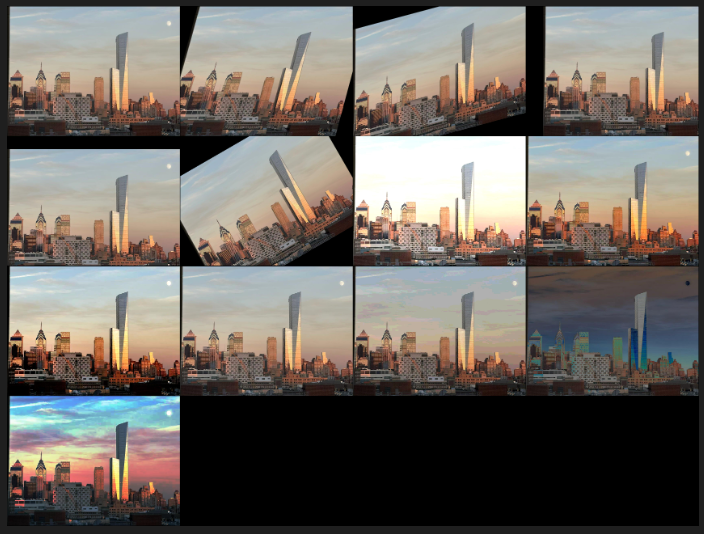
\includegraphics[width=0.95\textwidth]{figures/augment_examples.png}
    \caption{Visualization of image augmentation operations and their effects.}
    \label{fig:augment}
\end{figure}

\end{solution}

\clearpage

\begin{solution}[Time spent: 1 hours]
\paragraph{(a) Non-convexity.}
Consider the objective
\[
f(A,B) = \|X - AB\|_F^2.
\]
Let us take the scalar case \(m = n = r = 1\), so that \(x \in \mathbb{R}\) and \(a,b \in \mathbb{R}\).
Then \(f(a,b) = (x - ab)^2.\)
Choose \(x = 0\), and two points \((a_1,b_1)=(0,2)\) and \((a_2,b_2)=(2,0)\).
We have
\[
f(a_1,b_1)=f(a_2,b_2)=0,
\]
but their midpoint \((1,1)\) satisfies \(f(1,1)=1 > 0 = \tfrac12 f(a_1,b_1) + \tfrac12 f(a_2,b_2)\).
Hence \(f\) is not convex in the joint variable \((A,B)\).

\paragraph{(b) Global optimum and SVD.}
Let the singular value decomposition (SVD) of \(X\) be
\[
X = U \Sigma V^\top, \qquad \Sigma = \mathrm{diag}(\sigma_1, \sigma_2, \ldots, \sigma_p),
\]
where \(p = \min(m,n)\) and \(\sigma_1 \ge \sigma_2 \ge \cdots \ge \sigma_p \ge 0.\)
Let \(U_r, V_r\) contain the first \(r\) singular vectors and
\(\Sigma_r = \mathrm{diag}(\sigma_1, \ldots, \sigma_r)\).
By the Eckart--Young--Mirsky theorem, the best rank-\(r\) approximation of \(X\) is
\[
X_r = U_r \Sigma_r V_r^\top,
\]
and it satisfies
\[
\min_{\mathrm{rank}(AB)\le r} \|X - AB\|_F^2
= \|X - X_r\|_F^2
= \sum_{i=r+1}^{p} \sigma_i^2.
\]
Therefore any factorization \(A,B\) such that \(AB = X_r\) achieves the global minimum,
for example
\[
A^{\ast} = U_r \Sigma_r^{1/2}, \qquad B^{\ast} = \Sigma_r^{1/2} V_r^\top,
\]
or equivalently \(A^{\ast} = U_r \Sigma_r, \, B^{\ast} = V_r^\top.\)

\paragraph{(c) Uniqueness.}
The solution is generally not unique.
\begin{itemize}
  \item For any invertible \(R \in \mathbb{R}^{r\times r}\),
  \[
  A' = A^{\ast} R, \qquad B' = R^{-1} B^{\ast},
  \]
  gives the same product \(A'B' = AB = X_r.\)
  \item If the singular values satisfy \(\sigma_r = \sigma_{r+1}\),
  the optimal subspace \(U_r,V_r\) itself is not unique:
  any orthogonal rotation within the degenerate subspace yields another valid optimum.
\end{itemize}
When \(\sigma_r > \sigma_{r+1}\), the optimal matrix \(X_r\) is unique,
but its factors \(A,B\) remain non-unique up to the above linear transformation.
\end{solution}

\clearpage




\begin{solution}[Time spent: 5 hours]
Your solution goes here.\\
\end{solution}

\end{document}
